\section{Semantic Web}
Il Web Semantico è una rete di informazioni collegate tra loro in modo da essere facilemente interpretabili dai computer.
Ogni dato nel web semantico è rappresentato da un \textbf{URI} una stringa composta da due parti \texttt{<scheme>} e \texttt{<path>} che identifica in modo univoco la risorsa.

\subsection{RDF - Resource Description Framework}
RDF è una notazione per modellare informazioni nel web usando una tripa di URI con il seguente significato:
\begin{center}
\texttt{subject property object}
\end{center}
Ogni tripla associa ad un oggetto (\textit{subject}) una proprietà o verbo (\textit{property}) che ha un determinato valore (\textit{object}), un esempio di tripla RDF è dato da:
\begin{center}
\texttt{<http://example.com/rev1> <http://amk.ca/review\#subject> <urn:isbn:1930110111>}
\end{center}
e modella il fatto che la risorsa \texttt{http://example.com/rev1} è relativa all'oggetto \texttt{run:isbn;1930110111}.
I dati RDF possono essere scritti in due formati \textbf{XML RDF} e \textbf{Notation3} entrambi equivalenti, viene preferito Notation3 perché è più semplice e meno verboso di XML RDF.\\ 
Tra i vari vantaggi di Notation3 c'è la possibilità di usare i prefissi:
\begin{lstlisting}
<http://xyz.org/\#subject> <http://xyz.org/\#prop> <http://xyz.org/\#object>
\end{lstlisting}
Può essere scritto in modo più compatto come:
\begin{lstlisting}
@prefix xyz: <http://xyz.org/\#>
xyz:subject xyz:prop xyz:object
\end{lstlisting}
Comunemente sono usati questi prefissi:
\begin{itemize}
\item @prefix : $<$\#$>$ .
\item @prefix rdf: $<$http://www.w3.org/1999/02/22-rdf-syntax-ns\#$>$
\item @prefix rdfs: $<$http://www.w3.org/2000/01/rdf-schema\#$>$ 
\item @prefix dc: $<$http://purl.org/dc/elements/1.1/$>$ .
\item @prefix foaf: $<$http://xmlns.com/foaf/0.1/$>$ .
\end{itemize}
\texttt{dc} e \texttt{foaf} sono dei vocabolari per RDF contenenti delle proprietà e classi usate per descrivere documenti e persone, questi vocabolari sono identificati da un URL in modo da garantirne l'unicità nel web.

\subsubsection{Grafi}
Le informazioni date da un modello RDF possono essere aggretate in un grafo dove i nodi rapresentano le risorse o delle costanti e gli archi rappresentano le proprietà.
\begin{figure}
\centering
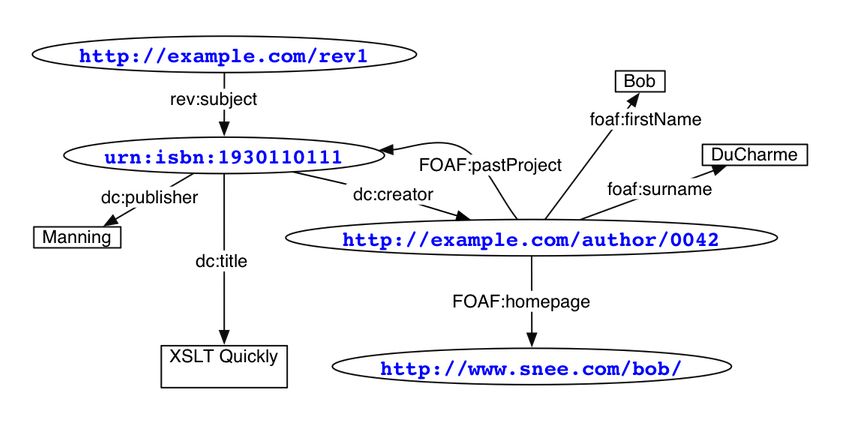
\includegraphics[width=0.8\textwidth]{images/sample_graph.png}
\caption{Esempio di grafo RDF}\label{fig:1}
\end{figure}

\subsection{RDF Schema}
Un RDF-Schema è un vocabolario per RDF che aggiunge sopra a RDF un sistema di tipizzazione, infatti con RDFS è possibile esprimere dei concetti come "Fido è di tipo Cane" e "Cane è sottotipo di Animale".
Ad esempio è possibile definire il vocabolario Pets come:
\begin{lstlisting}
@prefix pets: <http://example.com/xml/pets#> .
pets:Dog rdf:type rdfs:Class .
pets:name rdf:type rdfs:property .

:Fido rdf:type: pets:Dog .
:Fido pets:name "Fido" .
\end{lstlisting}
Oltre a questo RDFS permette anche di definire un dominio e un range di valori per le proprietà:
\begin{lstlisting}
#Impongo che la proprietà nome si possa associare solo a risorse di tipo pets:Dog e che possa avere solo valori di tipo stringa
pets:name rdfs:domanin pets:Dog .
pets:name rdfs:range rdfs:Literal .
pets:name rdfs:comment "Nome del cane" .
\end{lstlisting}
Allo stesso modo è possibile definire una classe come sottoclassi di un'altra:
\begin{lstlisting}
pets:Labrador rdfs:subClassOf pets:Dog
\end{lstlisting}
Grazie a RDF Schema possiamo quindi sapere quali classi esistono e quali proprietà hanno, però non esiste un modo per sapere quando due classi sono equivalenti.

\subsection{OWL - Web Ontology Langueage}
Permette di specificare che relazione c'è tra due oggetti/classi/proprietà appartenenti a vocabolari diversi, ad esempio
\begin{lstlisting}
gen:Person owl:equivalentClass foaf:Person
\end{lstlisting}
Per le proprietà, oltre all'equivalenza, è possibile anche speficare altre informazioni come \texttt{owl:inverseOf}, \texttt{owl:TransitiveProperty} e \texttt{owl:SymmetricProperty}.
Per due risorse è possibile specificare che siano la stessa cosa mediante \texttt{owl:sameAs}.

\subsection{SPARQL}
SPARQL è un linguaggio che permette di scrivere query per lavorare con i dati RDF, offre una sintassi SQL-Like e lavora solamente con RDF e RDFSchema questo garantisce di avere una ricerca che termini sempre, cosa che non sarebbe garantita se usasse OWL.\\
Un esempio di query che ritorna gli url dei blog di "Jon Foobar" è la seguente:
\begin{lstlisting}
PREFIX foaf: <http://xmlns.com/foaf/0.1/>
SELECT ?url
FROM <bloggers.rdf>
WHERE {
	?contributor foaf:name "Jon Foobar"
	?contributor foaf:weblog ?url
}
\end{lstlisting}
\begin{itemize}
\item La prima riga definisce il prefisso per il vocabolario/namespace in uso.
\item La seconda riga definisce che cosa la query deve ritornare, in questo caso la variabile \texttt{?url}. Da notare che in SPARQL le variabili possono iniziare con \texttt{?} o \texttt{\$}
\item la clausola FROM specifica dove eseguire la query, in questo caso è un file locale ma può anche essere un URL
\item Infine la clausola WHERE consiste in una serie di triple che definiscono il pattern da matchare sul grafo
\end{itemize}
\begin{figure}
\centering
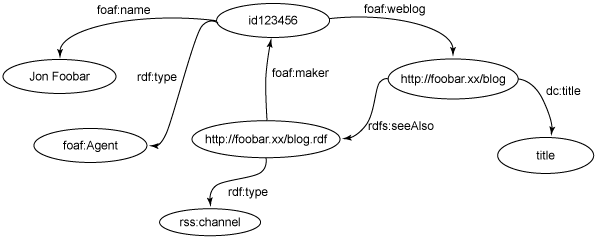
\includegraphics[width=0.8\textwidth]{images/blog_graph.png}
\caption{bloggers.rdf}\label{fig:3}
\end{figure}
Con SPARQL è possibile anche scrivere query molto più complesse sfruttando meccanismi come l'optional matching, l'alternative matching e i filtri che permettono di limitare le variabili, è inoltre possibile lavorare su più grafi contemporaneamente.
Per integrare SPARQL esistono dei framework come \textbf{Jena} che offrono delle API per Java.













